\chapter{Analysis}
\label{ch:analysis}
The main objective of this work is to build an extensible prototype,
which will be built on the model of visual attention and additionally
extended to classify
a set of images. This chapter discusses the main concerns
that have to be taken into consideration in order to achieve the objective.

Firstly, let's define the clear problem statement:

\textit{
	Given a dataset where each sample consist of a group of images.
	A certain label is asserted to every sample in a dataset. The goal is
	to build a extensible prototype upon \gls{RAM} that is capable of classifying
	this samples. The prototype is the resemblance of the \gls{RAM} model with
	with the ability to accept the above mentioned dataset.
}

\\

% TODO:
% * name the section regarding the quality
% * finish the Analysis chapter:
% ** what is best practices in python?
% ** what is best practices in general?
% ** Limitations of the preivous work> fullfil the lsit belowe

\section{Quality concerns}
\label{sec:quality_concerns}
This statement makes it clear that the prototype should be extensible. Extensible
means that other people(including author itself) are able to extend the
prototype. People should comprehend the code as well as the configuration
procedures in order to extend the prototype. Therefore, following the best practices
and conventions, using widely known frameworks, producing clean and readable code
to stay consistent with other modern software are  important
points of this work.

It's more convenient to talk about conventions once programming language and
libraries are chosen for this work.
\paragraph{TensorFlow}

There is a big variety of frameworks and libraries used in machine learning.
Among the famous libraries is library called TensorFlow. TensorFlow is an open
source library developed and maintained by engineers from Google \cite{tensorflow2015-whitepaper}.


TensorFlow framework has gained a huge popularity among machine learning
community as well as in industry compared to another framework \cite{DBLP:journals/corr/Goldsborough16}.
TensorFlow is an open source software library that makes computations more
efficient by building a computation graph and deploying them to one or more
CPUs or GPUs.


TensorFlow framework gives a wide variety of statistical distributions, wide
range of loss functions, and a huge amount of neural network algorithms while
not necessarily losing  flexibility. In order to make learning process traceable,
TensorFlow provides TensorBoard, which is a web interface for graph visualization
built directly into TensorFlow.
TensorBoard is an important and uniq feature that excels TensorFlow from similar
libraries; it improves debugging experience as well as helps
for understanding models that was developed using the TensorFlow.
Aforementioned features of the framework as well
as it's great API for Python is a great fit for this work.

The current work will use Python as programming language, as it's one of
the most popular languages among machine learning community.


\paragraph{Code conventions}
Now that we assigned interfaces, let's define the conventions that this work
will follow. As TensorFlow recommends using PEP 8 style guide, we will use it
as well to stay consistent
with community \cite{TfWeb}. PEP 8 gives the set of rules about how to layout
the code, how to name functions, methods and classes and others code style related
aspects \cite{Rossum}. PEP 8 linter is also integrated in the project, which checks the code
automatically on presence errors against PEP 8 style guide,
therefore simplifies the development workflow.

PEP 257 convention is also considered as this will help to avoid errors when
generating documentation. PEP 257 convention set rule about organizing
docstrings in Python \cite{Goodger2001}.
Overall, the work follows The Hitchhiker's Guide to Python, which advises
about the way of testing, organizing and documenting the code \cite{Reitz}.

\paragraph{Code patterns}

Despite that a lot of code from researches are not following and not using code
pattern, it really simplifies the understanding and reasoning about the code, especially
while extending or adjusting the model. Therefore using code patterns
is highly recommended. We will introduce the code patterns, which
is recommended in the functional programming from \cite{beck1997smalltalk},
because python supports the concept of functional programming.
To follow are also general well-known code patterns that are taken from
\cite{martin2003agile}, \cite{Eckel2017}, \cite{Gamma:1995:DPE:186897}.
Below is a list of this code pattern recommendations:

% design patterns
\begin{itemize}
	% done
	\item Composed method - it's saying that methods should
		have one identifiable task. Additionally to this, all operations
		performed in the function should be on the same level abstraction.
		This will increase flexibility of the methods and prevent
		from confusing code and mistakes. \cite{beck1997smalltalk}
	% done
	\item Extract method - when one method is too long, one should try to
		extract some part of it into another function taking into account that this
		function should be useful on its own. \cite{1999:RID:311424}
	% implement or throw it away
	\item Method object -  normally applied when one can't use extract method
	 	on a function because new function would take a lot of parameters
		from the original method.
		The idea is to create a small class that will hold the parameters
		as properties and then to create small methods within this class without
		passing the parameters to it, but instead access them as class properties.
		\cite{beck1997smalltalk}
	% implement
	\item Method comment - instead of having a comment close to not
		self-explanatory statement, one should rather create a function
		with self-explanatory name that holds this statement.
		Most comments are redundant, therefore one can simplify
		the system by introducing small methods.
		\cite{beck1997smalltalk}
	% done
	\item Temporary variable - instead of having very long expression, it's recommended
		to assign part of the expression to a variable. This variable can also have
		the self-explanatory name, consequently increasing the readability of the code.\cite{beck1997smalltalk}

	% \item Simple Enumeration Parameter - having a simple name of a parameter
	% 	when iterating over enumeration: \lstinline{for each in plugins:} \cite{beck1997smalltalk}
	% done below
	\item Cascade pattern - when a method of a class doesn't return any value,
		one can return instance of the class in order to be able to call a
		next method of the instance in cascade way: \lstinline{self.doThis().doThat()}.\cite{beck1997smalltalk}
	% done below
	\item Single responsibility principle - it forces every class to have only one
		clearly distinguishable responsibility.\cite{martin2003agile}
	% done
	\item Duck Typing - is a specifically to python, a design principle that
		says that if an object has a certain desired functionality it doesn't matter
		what of nature the object is.
	% % bullshit
	% \item Composition over inheritance - it's design pattern which obligates
	%  	to use composition rather than inheritance. \cite{Gamma:1995:DPE:186897}
	% done
	\item Iterator - is a design pattern that says to access values of a list
	 	without exposing the list \cite{Gamma:1995:DPE:186897}. It's built into python language itself and
		can be used with syntax like \lstinline{for .. in ..} or \lstinline{next()}.
	% done
	\item Singleton - design pattern that obligates a class to be
		instantiated only once. \cite{Eckel2017}
\end{itemize}

% keep a system decoupled and thus easier to refactor, change, and redeploy
% https://en.wikipedia.org/wiki/Separation_of_concerns
% https://refactoring.com/catalog/replaceMethodWithMethodObject.html
% https://refactoring.com/catalog/extractMethod.html
% http://codebetter.com/jeremymiller/2006/12/03/composed-method-pattern/
% inderact variable acces
Since ML programming is more method oriented, most patterns above concentrate
on how to keep functions readable, precise and flexible. In this work we will follow
these patterns.

We will see examples of those patterns in the \autoref{ch:design}
and \autoref{ch:implementation}.

To recap, the prototype should be not only a good start for making further
improvements on large scale objects but also be a piece of software that bears the
following properties: extensible, well documented, integrable with other
softwares, easy configurable, readable code.


\section{Analysis of the previous work}
As we will build the current model upon the \gls{RAM} described
in \autoref{sec:ram_model}, it makes sense to look over the existing implementations
of the \gls{RAM} model.
The authors of \gls{RAM} paper haven't provided the implementation, but
fortunately there are some implementations built by the open source community.
It's common to see that people, who are working on a model as open source project,
often do it in their free time. As a consequence, it is expected that those model
are not high-quality prototypes, therefore in order to rely on the project
one needs to be meticulous while choosing one.
This is the following criteria we're considering when choosing the model for the basis
of this work:

\begin{itemize}
	\item Structure and readability of the code - at least presence of the basic structure
	\item Configuration - it should be comprehensible how one can change parameters
		of the model
	\item Reproducible results
	\item Presence of basic documentation
	\item Framework - as we have already chosen TensorFlow, projects built upon
		TensorFlow are preferable.
\end{itemize}

After doing the research and taking into account the above listed criteria,
the choice fell on the project from github user 'zhongwen'. We will refer to
this implementation as \emph{
	basic \gls{RAM} implementation
	\footnote{The original project is located on github: https://github.com/zhongwen/RAM .}
}.

This project is built using TensorFlow framework.
% TODO: change the notation.
\subsection{Advantages over original RAM paper}
Building a machine learning software is not as straight forward as building
conventional software. In machine learning, in order to achieve high accuracy
one uses different methods which are normally hard to comprehend without knowing
the theory behind them. Absence of testing is another point which makes it
harder to understand others code. Considering the circumstances and careful
analyses the approaches used in the basic RAM implementation
is desired for the success of this work.

\paragraph{Inference} in the current work was performed differently from what was
described in \cite{DBLP:journals/corr/MnihHGK14}.
% The method used in \cite{DBLP:journals/corr/MnihHGK14} was to running
% $M$ episodes on the one sample following by updating the parameters of the network.
Let's take a look at how the gradient of objective function is calculated in \cite{DBLP:journals/corr/MnihHGK14}:
\begin{equation} \label{eq:}
	\Delta_{\theta} J = \frac{1}{M} \sum_{i=1}^M \sum_{t=1}^T
		\Delta_{\theta} \log \pi_{\theta}(a_t^i| s_t^i) (R_t^i - b_t)
\end{equation}
where $J$ - is a cost function, $M$ - number of episodes,
$T$ - is a time step where the agent is forced to make a classification decision(end of an episode),
$s_t^i$ - state at time step $t$ of episode $i$,
$b_t$ - baseline to reduce variance, $a_t^i$ - action at time step $t$
of episode $i$.

As we can see the gradient is calculated based on running $M$ episodes.
Firstly, the agent chooses sequentially $T$ locations and finally makes a classification
decision. Then we run $M$ similar episodes like this. After this,
we compute the gradient. The basic RAM implementation used slightly different
approach. It does not run multiple episodes to update the parameters, but instead
it does update parameters on every episode. However it duplicates the same
samples $M$ times and then obtain $M$ different outputs and average them.
This practice was introduced in \cite{DBLP:journals/corr/BaMK14}.
It was also indicated that running attention model multiple times on each
image with the classification predictions being averaged gave the best
performance \cite{DBLP:journals/corr/BaMK14}.


\paragraph{Adam Opmitimizer} It also worth to notice that instead of stochastic
gradient descent that was used in RAM paper, the basic RAM implementation using Adam optimizer
from \cite{DBLP:journals/corr/KingmaB14} with exponentially decaying learning rate,
which theoretically should improve performance. \cite{DBLP:journals/corr/KingmaB14}


\paragraph{Gradient clipping} In contrast to RAM paper, the basic RAM implementation
additionally clipped the gradient values by global norm of their values.
This is normally done to prevent the vanishing
and the exploding gradient problems \cite{Pascanu2012}.


\subsection{Limitations}
Unfortunately, the basic RAM implementation used old version of TensorFlow,
which was unstable at that moment, therefore migration of the project
to the latest TensorFlow version is required\footnote{
	Migration was performed according to the TensorFlow migration
	guide: https://www.tensorflow.org/install/migration
}.

Looking at basic RAM implementation purely from software engineering side,
one can observe several flaws. Not following python conventions as well
as lack of design patterns and partial presence of incoherent structures in the code
are known obstacles when analyzing and extending the code.
Therefore code is required to be refactored and cleaned,
as well as restructured and documented under the conventions and
practices described in \autoref{sec:quality_concerns}.

% It's very common to see that researchers don't worry much about the
% building well-engineered prototype as most of them are not software engineers.
% Mostly the are big experts at math, it's understandable since excelling both
% fields is very time consuming. The basic RAM implementation is not an exception.
% The code is required to be refactored and cleaned, as well as restructured.

As for functional requirements, the lack of one feature was detected in basic RAM implementation.
As you can remember from \autoref{sec:ram_model}, glimpse sensor is taking
multiple patches from an image, where each patch is taken at different resolution.
The basic RAM implementation is not capable of taking multiple patches,
but only a single one. Without the ability of taking multiple patches within a glimpse,
accuracy of inference will be more likely to decrease when working with high-resolution
images.

Additionally to this, TensorBoard wasn't configured in basic RAM implementation.
Training such massive model as RAM can be complex and sometimes confusing.
Tools like TensorBoard make models easier to understand, debug
and optimize, therefore having fully configured TensorBoard is another
prerequisite for a good prototype.




% TODO for tomorrow:
% * revise the paragraph above, be precise and careful and think about all problems/ DONE
% * limitations are important, also say that everything below is opinionated and / DONE
	% a this a pure look from software engineering side
% * write about probably about the importance of the design patterns()
% * finish the analysis




% Original project contained
% a lot of style errors and had many inconsistencies in the code with respect
% to code style.
% The code is not followed by conventions therefore one can notice

% tesnorflow version
% tensorboard
% structure
% was not suitable for taking multiple patches
% very start level of documentation
% Absence of basic documentation


% \paragraph{paragraph name}









% \paragraph{Analysis}



% Machine learning is a field where
% But before actually building the extension upon this project,
%
%
% can have lack of documentation and b
% This can be a reason for having
% due to lack of resources
% As the implmentations provided by open source community
% often have lack of documentation and
%
% One of them due to certain level of readability is more attractive for this work.
% While the project is way more readable compared to others, it's still in the need
% of refactoring.
% This code is implemented by using tensorflow framework.


\section{Extension}
\label{sec:extension}
In order to fulfill the objective of this work, it's required to extend the basic
RAM implementation in a following way: it should accept a group of images as input
and based on that input make a classification decision. Group in this case means
more than one image(e.g. 2, 3 or 5 images and etc.). More formally:
\textit{given a group of images, extended model returns a probability distribution over
$K$ different outcomes, where $K$ - is amount of classes in the classification problem.}
We'll refer to amount of the image in a group as $n$.

This section will discuss several ways of how to achieve that.
In the figure \ref{fig:ram_model_arch} you can see original architecture of RAM.
The potential extension variations listed below will use the notation, which
was presented in \autoref{sec:ram_model}.

\begin{figure}[h!]
	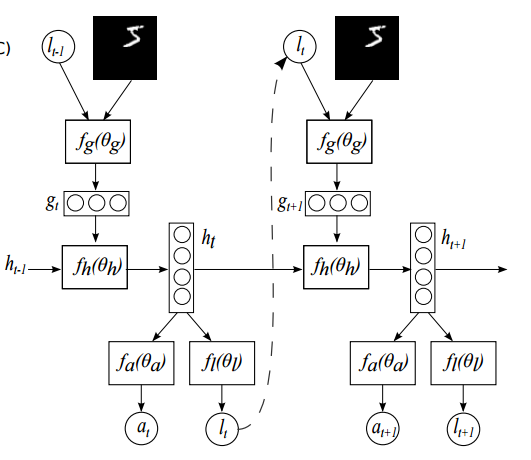
\includegraphics[width=\linewidth,scale=0.4]{ram_model_arch}
	\caption{Original architecture of RAM (source: \cite{DBLP:journals/corr/MnihHGK14}).}
	\label{fig:ram_model_arch}
\end{figure}

\subsection{Picker network}
\label{subs:picker_net}
You might remember the output of LSTM cell $h_t$ in \cite{DBLP:journals/corr/MnihHGK14}
which was described in \autoref{sec:ram_model}.
The external output is used
in the action network $f_a(\theta_a)$ as well as in location network $f_l(\theta_b)$
as shown in figure \ref{fig:ram_model_arch} to produce a classification decision or
next location respectively. In a similar way, we can invent a new network that takes as
input the LSTM cell's output $h_t$, have parameters $\theta_p$ and outputs
the probability distribution over $n$. We shall call this network
\emph{picker network}. The purpose of the picker network is to pick an image
in the group to explore appropriate image, hence the name. By manifesting
this extension, the model as a whole will have three neural networks consuming
the output of LSTM cell $h_t$:
\begin{itemize}
	\item Classification network $f_a(h_t; \theta_a)$ - makes a classification
		decision after $T$ number of time steps.
	\item Location network $f_l(h_t; \theta_l)$ - decides where to allocate the next glimpse
	on the picture.
	\item Picker network $f_p(h_t; \theta_p)$ - decides what picture to allocate the next glimpse on.
\end{itemize}

All of networks above have a similar structure:
\begin{align} \label{eq:picker_network}
	f_a(h_t; \theta_a) = Softmax(Linear_{\theta_a}(h_t)) \\
	f_l(h_t; \theta_l) = Linear_{\theta_l}(h_t) \\
	f_p(h_t; \theta_p) = Softmax(Linear_{\theta_p}(h_t))
\end{align}
wher $Softmax$ - is softmax activation function
$Linear_{\theta}(x)$ - represents
a linear transformation $Linear_{\theta}(x) = W_{\theta}x+b_{\theta}$ with weights
$W_{\theta}$ and bias $b_{\theta}$.


\subsection{Deep attention model}
\label{subs:deep_att_model}
This idea was inspired by the approach used in \cite{DBLP:journals/corr/BaMK14}.
The idea is to completely separate classification network from location network
by introducing new RNN layer on top of the current RNN layer.

\begin{figure}
	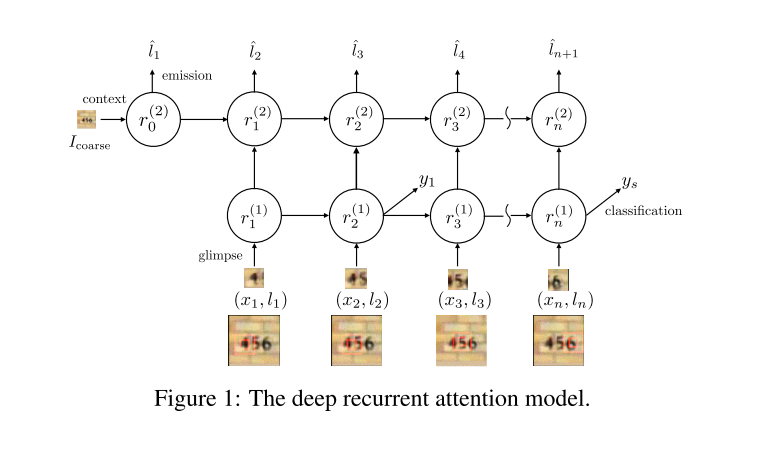
\includegraphics[width=\linewidth,scale=0.7]{deep_attention_model.png}
	\caption{The deep recurrent attention model (source: \cite{DBLP:journals/corr/BaMK14})}
	\label{fig:deep_att_model}
\end{figure}

In figure \ref{fig:deep_att_model} you can observe first RNN denoted $r^{(1)}$ which works
the same way as was described in \autoref{sec:ram_model}. Output of RNN $r^{(1)}$
was consumed by the location network and classification network in \cite{DBLP:journals/corr/MnihHGK14}.
This will be different in current approach. We can describe it as following:
We introduce new RNN $r^{(2)}$ on top of first RNN:
\begin{itemize}
	\item The new \gls{RNN} is initialized by output from convolution
		network(called Context Network) applied on the down
		sampled low-resolution version of input image.
		The feature vector outputted from convolutional layer
		provides sensible hints on where
		the potentially interesting regions are.
		The reason behind it was described in \cite{DBLP:journals/corr/BaMK14}:
		\blockquote{The existence of the contextual information(feature vector),
		however, provides a
		“short cut” solution that is much easier for the model to
		learn from contextual information than by combining information
		from different glimpses}
	\item The new \gls{RNN} takes as input the output of \gls{RNN} $r^{(1)}$:
		$r_n^{(2)} = f_{r^{(2)}}(r_n^{(1)}, r_{n-1}^{(2)})$,
		where $r_n^{(1)}$ - is the output of \gls{RNN} $r^{(1)}$ at time step $n$,
		$f_{r^{(2)}}$ - is \gls{RNN} cell function of the new \gls{RNN} $r^{(2)}$ (e.g. \gls{LSTM} cell),
		% $r_n^{(2)$ and $r_{n-1}^{(2)}$
		  $r_n^{(2)}$ and $r_{n-1}^{(2)}$ are outputs of \gls{RNN} $r^{(2)}$
		  at time step $n$ and $n-1$ respectively.
	\item The output of new \gls{RNN} is used to produce next location.
		The output is fed into fully connected network, which maps
		the feature vector produced by new \gls{RNN} into coordinate object $[i, (x,y)]$,
		where $i$ - is a index in the group of images. Having this index $i$,
		which can be from $0$ to $K$, we attend to a certain image $i$ at the location $(x, y)$.
\end{itemize}

The reason for having the second \gls{RNN} is to implicitly
represent decision about location and
prevent using location information in classification. Separation is crucial:
first \gls{RNN} network is responsible for
classification, while second one for choosing the right location.
One state will hold information about classification, while the state of
the \gls{RNN} cell on the top will hold information about locations.
One advantage of this work is that having this separation of concerns between
location and classification information which theoretically should improve the model.
We will refer to this approach as \emph{deep attention model}.

\subsection{Exploration network}
In original RAM paper, the model is required to execute a number of
steps before making classification decision:
\blockquote{
The attention network used in the following classification experiments made
a classification decision only at the last timestep $t = N$.
}\cite{DBLP:journals/corr/MnihHGK14}
It was also suggested as a further improvement to introduce new action
which decides when model should stop taking further glimpses:
\blockquote{
Finally, our model can also be augmented with an additional action that decides
when it will stop taking glimpses. This could, for example, be used to learn a
cost-sensitive classifier by giving the agent a negative reward for each glimpse
it takes, forcing it to trade off making correct classifications with the cost of
taking more. \cite{DBLP:journals/corr/MnihHGK14}
}

We can alter this suggestion by introducing a new action which
instead of indicating when the model should stop taking new glimpse, will
indicate when the model should take a next image in a group. Once there is no more images
we can force the model to make a classification decision.

We introduce a new network which takes an input of the state of RNN cell, and outputs
probability distribution over two actions which correspond to whether the model
will stop taking new glimpses
or continue to explore image.
We shall call this network \emph{the exploration network}.

By manifesting
this extension, similar to the approach described in \autoref{subs:picker_net},
the model will have three neural networks consuming
the output LSTM cell $h_t$:
\begin{itemize}
	\item Classification network $f_a(h_t; \theta_a)$ - makes a classification
		decision after $T$ number of time steps.
	\item Location network $f_l(h_t; \theta_l)$ - decides where to allocate the next glimpse
	on the picture.
	\item Exploration network $f_e(h_t; \theta_e)$ - decides whether the next glimpse
	should be taken
	from the $i$ image from the group or from the $i+1$ image.
\end{itemize}

New exploration network computes the distribution in the following way:
\begin{equation}
	f_e(h_t; \theta_e) = Softmax(Linear_{\theta_e}(h_t))
\end{equation}

The advantage of this approach is the flexibility since it can easily be combined
with deep attention model introduced in \autoref{subs:deep_att_model}. This
approach can be also augmented with following actions:
\begin{itemize}
	\item First Action - go back, that is, take previous image from the group of images.
	\item Second Action - go forward, that is, take next image from the group of images.
	\item Third Action - finish, that is, stop taking glimpse and do the classification decision.
\end{itemize}

There is no theoretical to prove which one from the extensions will work better,
therefore testing them with experiments is required.
We will chose only one of the approaches for
performing experiments since testing all the extensions
is out of scope of this work.

\section{Dataset}
\label{sec:analysis_dataset}

Before starting the construction of the model, one requires to think about an appropriate
dataset on which the model can be tested.
MNIST dataset\footnote{The MNIST data is hosted on \cite{LeCun2010}} is recognized
as being the simplest dataset among the computer vision
community, therefore building a dataset upon it would be easier. The simplicity of dataset
would help to understand problems occurring while developing a model.
Additionally to this, researchers from google
Deepmind used MNIST to evaluate RAM, which indicated that MNIST data would
be good fit for the extension as well. \cite{DBLP:journals/corr/MnihHGK14}


\paragraph{MNIST Dataset} MNIST dataset consist of scanned handwritten images, each labeled
from from set: $\mathcal{A} = \{0 .. 9\}$, where $\mathcal{A}$ - is a set of available
classes in MNSIT dataset. You can see an example of 4 digits in figure \ref{fig:mnist}.
Additionally, it includes a label for each of the image.

\begin{figure}[h!]
	
\includegraphics[width=\linewidth,scale=0.4]{MNIST}
	\caption{MNIST example (source: \cite{tensorFlowSite})}
	\label{fig:mnist}
\end{figure}

For example, in the figure \ref{fig:mnist} the labels are 5, 0, 4 and 1.
Each images consist of $28\times28$ pixels, hence an MNIST image would
be an array of size $784$.

MNSIT dataset consist of 55,000 training samples, 10,000 test samples, 5,000 validation samples.

\subparagraph{Group dataset}

Requirement for the new dataset can be formulated as following:\\
\textit{Each sample in the dataset should contain fixed number of images. Amount of images
in an sample should be more than 1. The dataset should have at least two classes,
which are used to label each of the sample. The dataset should provide enough
data to train, validate and evaluate the model.}



% There is different variations for building the dataset of group of images from MNIST dataset.
% One of them can be as simple as bringing two different numbers together and adding a
% noise image, which shouldn't have an influence on the outcome.
\subparagraph{Procedure}
We should come up with the dataset that will fulfill the requirements above.
One way of doing it could be described as following:
having limit of 10 classes in MNIST dataset, we decide about the class(or classes) of images
that hold information relevant for classification decision(it can be for example classes
labeled with 4 and with 3 in MNIST),
we'll refer to those images as non-noise images. Subset of classes of non-noise image
we denote as: $\mathcal{D} = \{d_1,..., d_n\}$.
We'll have also images which do not
contain any information relevant for decision making, we'll refer to this images
as noise images. Noise images are generated using images from classes that
are mutually exclusive with classes of non-noise images:
$\mathcal{T} = \mathcal{A} / \mathcal{D}$, where $\mathcal{T}$ - is a subset of classes $\mathcal{D}$
for labeling noise images: $\mathcal{T}\subset \mathcal{D}$.
% However, it's possible that $\not\subset$ TODO: finish it.
We then decide about the amount the images in a group $n$.
We then choose the number $k < n $ which is going to be amount of noise images
per sample in dataset.

% we choose one(or more) from this images(f.e. example image) and will call it(them) noise image(s) and refer
% to the amount of noise images as $k$.

We then divide the original MNIST dataset into two:
\begin{itemize}
	\item First dataset - consisting of noise images, where each sample is a group(array)
		of noise images with the size of $k$.
	\item Second dataset - consisting of non-noise images, where each sample is a group(array)
		of non-noise images with the size of $n-k$.
\end{itemize}

We then create a new dataset and fill the sample that is a concatenation of sample
from first dataset with sample of second dataset described above.
This way we're getting a new dataset
where each sample has a size of $n$. Using this method we can create two datasets with
different $k$, but the same $n$ and label them as dataset of first class, and
dataset of second class.

The conceptional idea behind this dataset, the the model should learn to
understand that noise image and that it does not bring any information relevant for the task.
Practical solution for classification task of this dataset would be
to understand what non-noise images are,
count them, and depends on the amount of non-noise images,
classify the sample
. If the model work correctly on this dataset, it will confirm
 that the model works correctly
for identifying images that are irrelevant for decision making

\section{Testing}
It's well-known that unit testing in ML models is not as trivial
as in conventional software,
therefore unit testing should be applied to only one part of the code where
behaviour is fully predictable. One such example for unit testing would to
check whether
certain components of the system having expected shape of vectors and matrixes.
As code for producing the dataset having procedural structure,
it should be fully tested in order to avoid
unexpected behaviour in the model.
\\
In this work, we will mostly concentrate on bringing this model to life,
therefore performance of the model does not play significant role.
But in order to get an idea of how well the model is performing and
to be able to analyse it, we will consider following performance metric:
accuracy on training, validation and test data, hybrid loss value and it's parts
and the cross entropy between ground truth and prediction. Additionally,
we will look at the time that the model taken to perform certain
amount of iterations.

% we need take extra care of this
% as to assure that the model works correctly.

% shdbasd
% It was de
%
%
% what is testable and what is not? like classes and shit

% in bachelor/implemntation,  http://python-guide-pt-br.readthedocs.io/en/latest/writing/structure/
% there is written a lot about:
% * structure
% * testing
% * pep008

% about why did you choose tensor flow

% In this chapter will be discussed the relation current work
% to previous work

% *Anwendung von Prinzipien, Methoden, Techniken und
% Werkzeugen der Informatik* in einem Anwendungsbereich zum
% Gegenstand haben.

% System- und Anforderungsanalyse, Beschreibungen von
% Systemfunktionen, -dynamik, -daten, -oberfläche,
% Schnittstellendefinitionen, Festlegungen zu Qualitätsparametern

% Bewertung von theoretischen Ansätzen, Konzepten, Methoden,
% Verfahren; informelle
% Aufgabenbeschreibung, klar formulierte Zielstellung;


% introduction to the chapter
%
% make a clear statement of the problem
% data
% Analysis of the problem
% current data is needed to be extended
% analysis of the existierte projects
% whaat is needed to be done to make the
% what will make the project great
% tested what can be tested, shapewise. Using what?
% tensorboard, the training should be trackable
%


% DATASET
% MNIST dataset is recognised as being the simplest dataset among the neural
% network community, hence building a dataset upon it would be easier. The
% simplicity of dataset would help to understand problems occurring while developing
% a model. There can be different variations for building a group of images to
% classify from MNIST dataset. One of them can be as simple as bringing two
% different numbers together and adding a noise picture, which shouldn't have
% an influence on the outcome. For example: [1,0,2] will be the  first class
% and [0, 3, 1] will be the second class. 0
% represents noise in this example and



%
% pay attention to TensorBoard since one of the objective of the thesis is to
% make training experience trackable.
% * provide a good overview of outcome. outcome should be as clear as
%  possible.
% * IMPORTANT: you should be able to see in a good and understandable way
%  the selection path of the model. That is, exactly how is it in the original paper.
%  That is, which image is chosen, which part of the image is chosen and etc.
